
\chapter{Decoder HW Architecture}

\section{Introduction}
This section is an overview of the design for the hardware accelerated PLVD programming logic (PL) and explanations behind the optimizations implemented. The design is heavily based on Chester Hulse’s initial design \cite{ChesterPaper} who similarly details many of the following optimizations. This section will expand on Section IV of his paper and detail the specific improvements made to the original design. 

\TODO{Correct cite}

\section{Hardware Optimizations}

\subsection{Metric Computation}
In PLVD, the computation of edge metrics is heavily repeated and constitutes a large portion of the computational complexity of the algorithm. The following simplifications can be made to metric computations, drastically reducing the complexity of the algorithm. 

As described in the PLVD algorithm, at each time point t, we compare the k bits of received message at time point $t$ with the encodings given by every edge in the trellis at that $t$. 
For $R = (R_i, \ldots , R_k)$ and $C = (C_1, \ldots, C_k)$ with $R$ representing the log likelihoods of the received bits $X = (X_1, \ldots, X_k)$ (for BPSK $R_i = \log( \frac{P(U_i = 0 | X_i)}{P(U_i = 1 | X_i)})$ ) at some time point and $C$ being the correct encoding corresponding to that edge, we deem the ML code word to be one that minimizes the following
$$ \min_C \sum_i {(R_i - C_i)}^2 $$

This is akin to measuring the Euclidean distance, but we make the following simplifications that make the metric calculation much more realizable in hardware. The square terms can be disregarded ed since they are constant for each given time point. So we have the following
$$\min_C \sum_i -2 R_i C_i $$

Finally we can drop the -2 and maximize instead of minimize
$$\max_C \sum_i R_i C_i $$

This simplifies updating the edge metrics associated with a path at a time point to just adding the bit LLRs whose corresponding encoding bit is a $0$ and subtracting the LLRs who’s bit corresponds to a 1. An example is shown below

Ex. in a rate $\frac{1}{5}$ code we update path metric $m$ at time point $t$ with respect to received LLRs $R = (R_0 R_1 R_2 R_3 R_4)$ and edge weight (encoding) $11010$.
$$m = m - R_0 - R_1 + R_2 - R_3 + R_4$$

Furthermore, in this type of code, two edges that leave the same node necessarily have inverse encodings. Thus in the previous example, the other edge will have weight $00101$ and path metrics can be updated as
$$m = m + R_0 - R_1 - R_2 + R_3 - R_4$$

\subsection{Merge Sort}
Another expensive and repeated operation in PLVD is the storage and filtering of the list of best paths at each iteration. In particular, choosing the $L$ best paths from two unsorted lists of size $L$ is very difficult on a hardware level. To remedy this, our implementation stores the $L$ paths sorted by their metrics. The task is now simplified to choosing the $L$ best paths from two sorted lists of size $L$ and we proceed as follows:

\vspace{5pt}

Let $l_1, l_2$ be the two sorted lists of $L$ paths to be filtered. Repeat the following a total of $L$ times to obtain a sorted list $l'$ of the $L$ best paths.
\begin{enumerate}
    \item Compare the top elements of $l_1$ and $l_2$, and select the path $p$ with the better metric
    \item In $l'$, place $p$ directly after the most recently added element
    \item Remove $p$ from future consideration from $l_1$ or $l_2$ respectively
\end{enumerate}

%%%%%%%%%%%%%%%%%%%%%%%%%%%%%%%%%%%%%%%%%%%%%%%%%%%%%%%%%%%%%%%%%
% FIGURE: Decoder HW: Merge Sort
\begin{figure}
\centering\CaptionFontSize
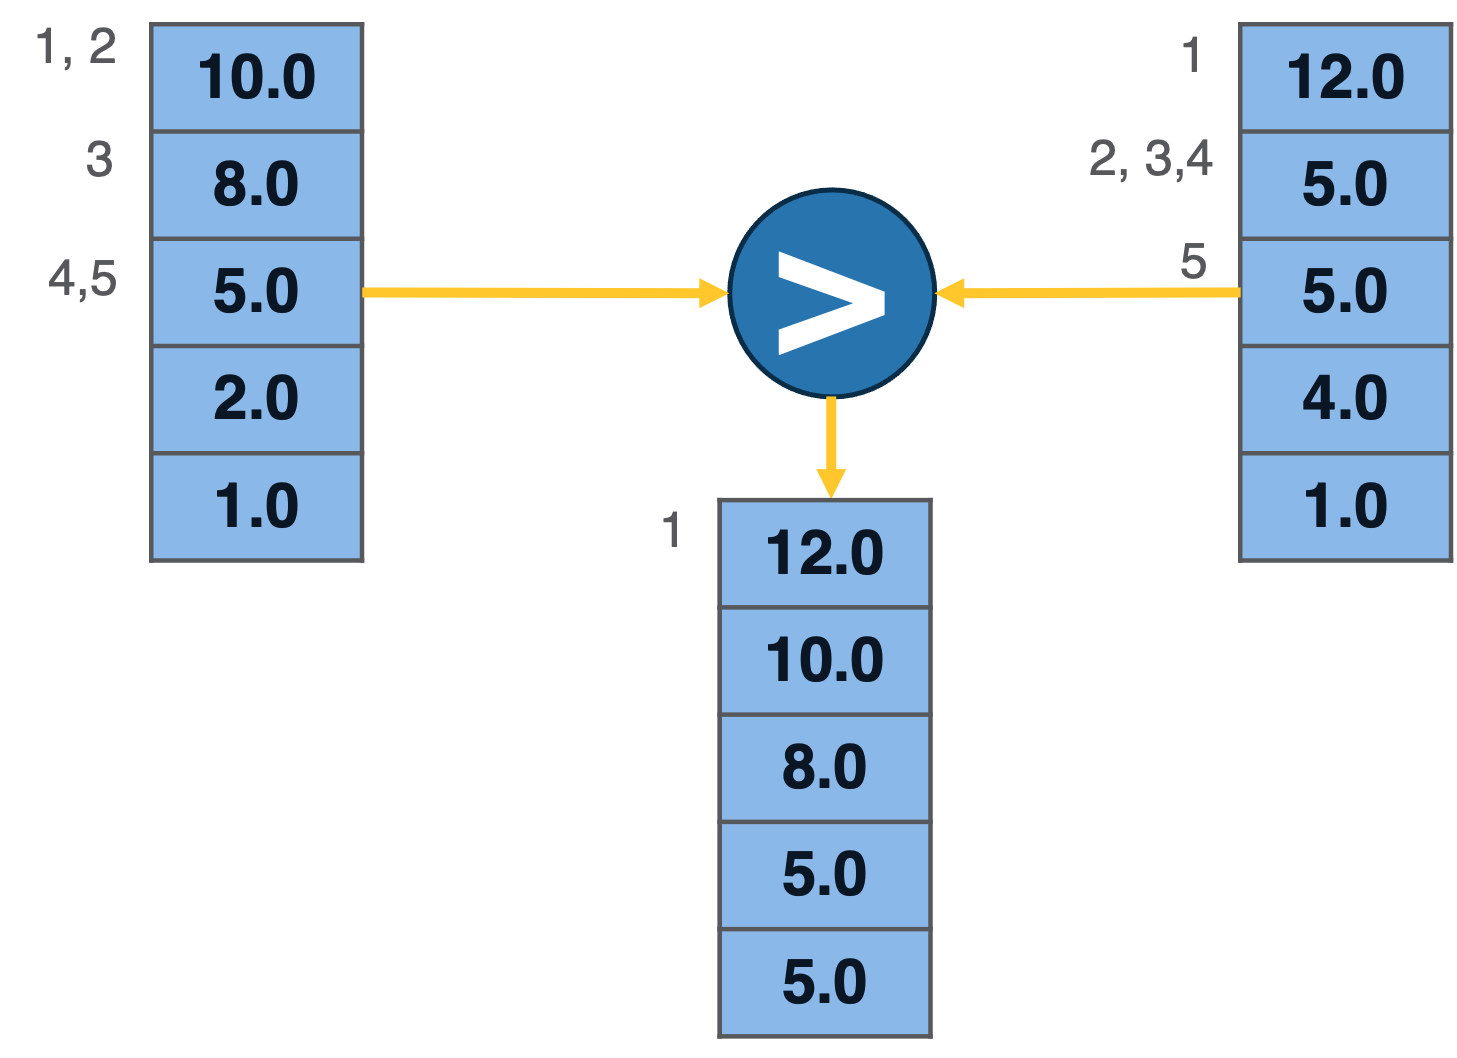
\includegraphics[height=15em]
{Figures/merge_sort.png}
\caption[Diagram detailing the merge sort sorting and storage of lists]
{Diagram detailing the merge sort sorting and storage of lists. Here $l_1$ and $l_2$ are shown with list lizes $L=5$. The numbers stored represent the path metrics (in reality there is more data stored in memeory) and the top values of the memory elements are always compared. Next to each entry is the iterations of the algorithm in which that value was examined for comparison.}
\label{Figure:DecoderHW:MergeSort}
\end{figure}
%%%%%%%%%%%%%%%%%%%%%%%%%%%%%%%%%%%%%%%%%%%%%%%%%%%%%%%%%%%%%%%%%

Note: from a data structures perspective, using a FIFO makes a lot of sense here, however, as we’ll see later, this actually ends up being more restrictive than we’d like.

\section{Hardware Architecture}
The overall architecture of the PLVD accelerator can be seen in \Figure~\fref{Figure:DecoderHW:OldArchitecture}. In this section we will discuss each module in detail. Aside from the LVA module, most others underwent minimal change from Hulse’s implementation \cite{ChesterPaper}, regardless, we explain for clarity.
\TODO{cite}

%%%%%%%%%%%%%%%%%%%%%%%%%%%%%%%%%%%%%%%%%%%%%%%%%%%%%%%%%%%%%%%%%
% FIGURE: Decoder HW: Old design architecture
\begin{figure}
\centering\CaptionFontSize
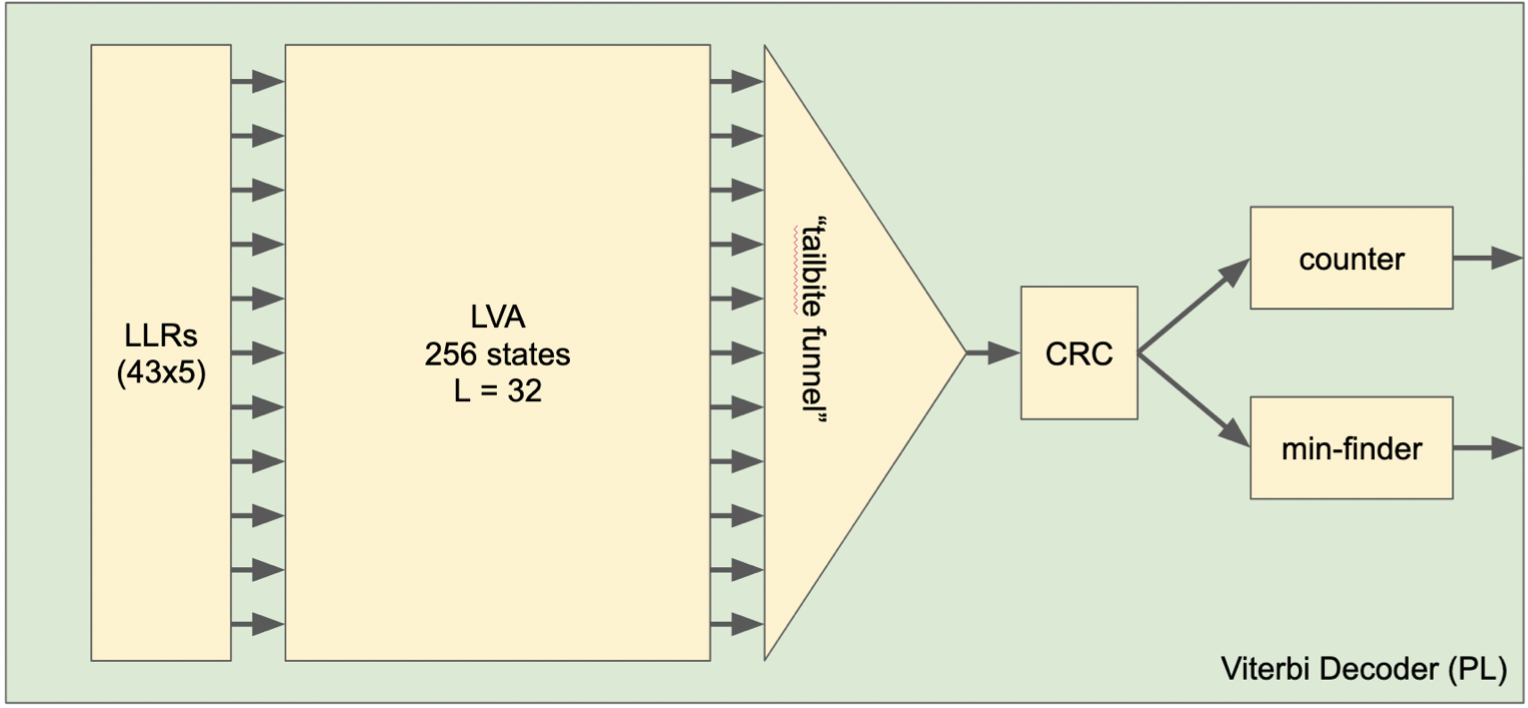
\includegraphics[height=15em]
{Figures/old_architecture.png}
\caption[Chester Hulse's design of FPGA PLVD]
{Chester Hulse's design of FPGA PLVD. Figure taken from \cite{ChesterPaper}}
\label{Figure:DecoderHW:OldArchitecture}
\end{figure}
%%%%%%%%%%%%%%%%%%%%%%%%%%%%%%%%%%%%%%%%%%%%%%%%%%%%%%%%%%%%%%%%%

The AMBA-AXI Stream interface is used to connect all modules where the data payloads are path objects as described below. AXI-Lite is used to handle fixed address memory access. 
\TODO{cite picture}
Input LLRs which represent the received code are stored in memory and serve as inputs for the LVA module. The LVA module runs PLVD as described above and outputs the L best paths through the trellis for each end state. The tail biting funnel module takes in parallel streams of paths and outputs a stream of paths that satisfy the TB condition. This stream is then passed through the CRC module that outputs the decodings that pass the CRC check. The decoding with the best metric is then chosen as the decoding of choice.

\subsection{Path Object}
This is the data structure used throughout the design that represents stores information about a path in the trellis. This is the data that is being written to memory and passed between modules via AXI. It holds 72 bits worth of data designed to maximize the width offered by BRAMs on a Xilinx ZCU106 board. Since we are investigating an 8 state, code with 43 transmitted bits, the data is structured as seen in \Figure~\fref{Figure:DecoderHW:PathObject}.

%%%%%%%%%%%%%%%%%%%%%%%%%%%%%%%%%%%%%%%%%%%%%%%%%%%%%%%%%%%%%%%%%
% FIGURE: Decoder HW: Path Object
\begin{figure}
\centering\CaptionFontSize
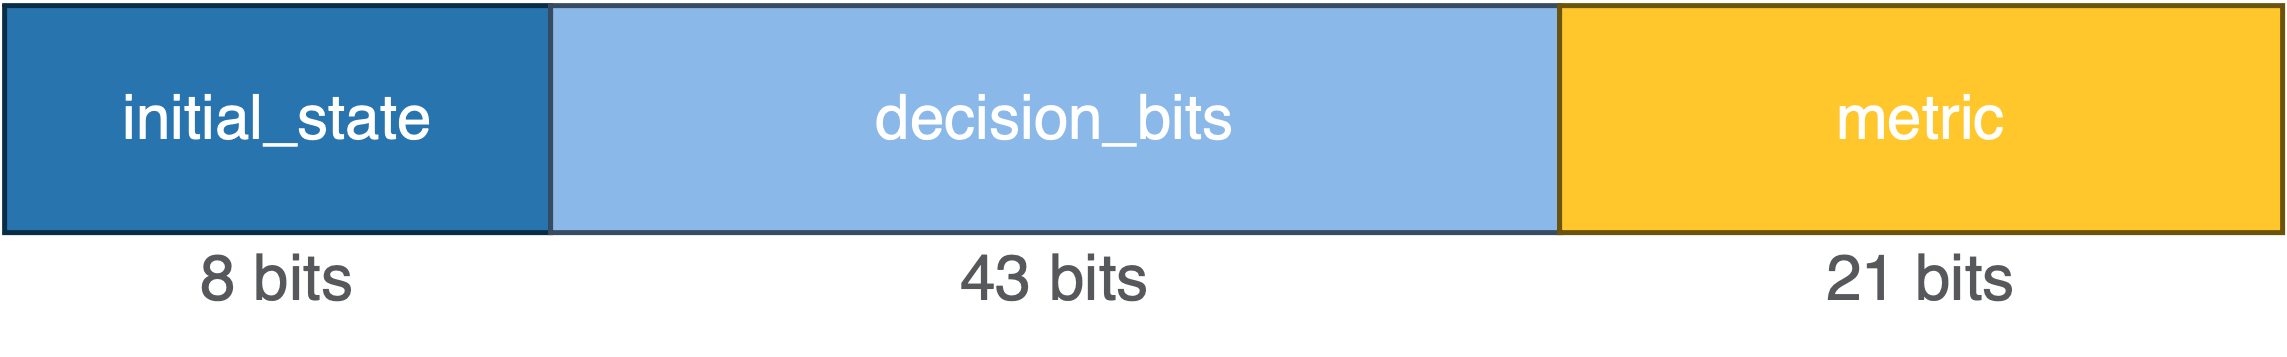
\includegraphics[width=\textwidth]
{Figures/path_object.png}
\caption[Diagram detailing the merge sort sorting and storage of lists]
{Diagram detailing the merge sort sorting and storage of lists. Here $l_1$ and $l_2$ are shown with list lizes $L=5$. The numbers stored represent the path metrics (in reality there is more data stored in memeory) and the top values of the memory elements are always compared. Next to each entry is the iterations of the algorithm in which that value was examined for comparison.}
\label{Figure:DecoderHW:PathObject}
\end{figure}
%%%%%%%%%%%%%%%%%%%%%%%%%%%%%%%%%%%%%%%%%%%%%%%%%%%%%%%%%%%%%%%%%

The “initial state” and “decision bits” elements give information on which path we are keeping track of while the “metric” element is the value that keeps track of the metric distance of the path with the received message. The size of the first two are fixed given the parameters of the convolutional code being transmitted, however, the number of bits used to calculate the metric was set to maximize the 72 bit structure of the BRAMs and can be changed as desired.

\subsection{LVA Module}
This module is the computational core of the decoder architecture which performs the PLVD algorithm. 
\subsubsection{Overview of Changes}
Hulse’s original design of the LVA core is in \Figure~\fref{Figure:DecoderHW:OldLVAModule}. Here, each state and edge in the state diagram has its own module; meaning at every time point, computations in steps 2a,b,c of the PLVD algorithm are done in parallel for every state; the design’s execution time depends only on the list size $L$ and the length of the code $T$. Furthermore, each state module uses two FIFO memory elements to store the incoming $L$ edge paths in order to implement the storage optimizations mentioned earlier. To implement these FIFO memory elements we ideally want to utilize high speed Programming Logic (PL) side Block Ram (BRAM).

%%%%%%%%%%%%%%%%%%%%%%%%%%%%%%%%%%%%%%%%%%%%%%%%%%%%%%%%%%%%%%%%%
% FIGURE: Decoder HW: Old LVA Module
\begin{figure}
\centering\CaptionFontSize
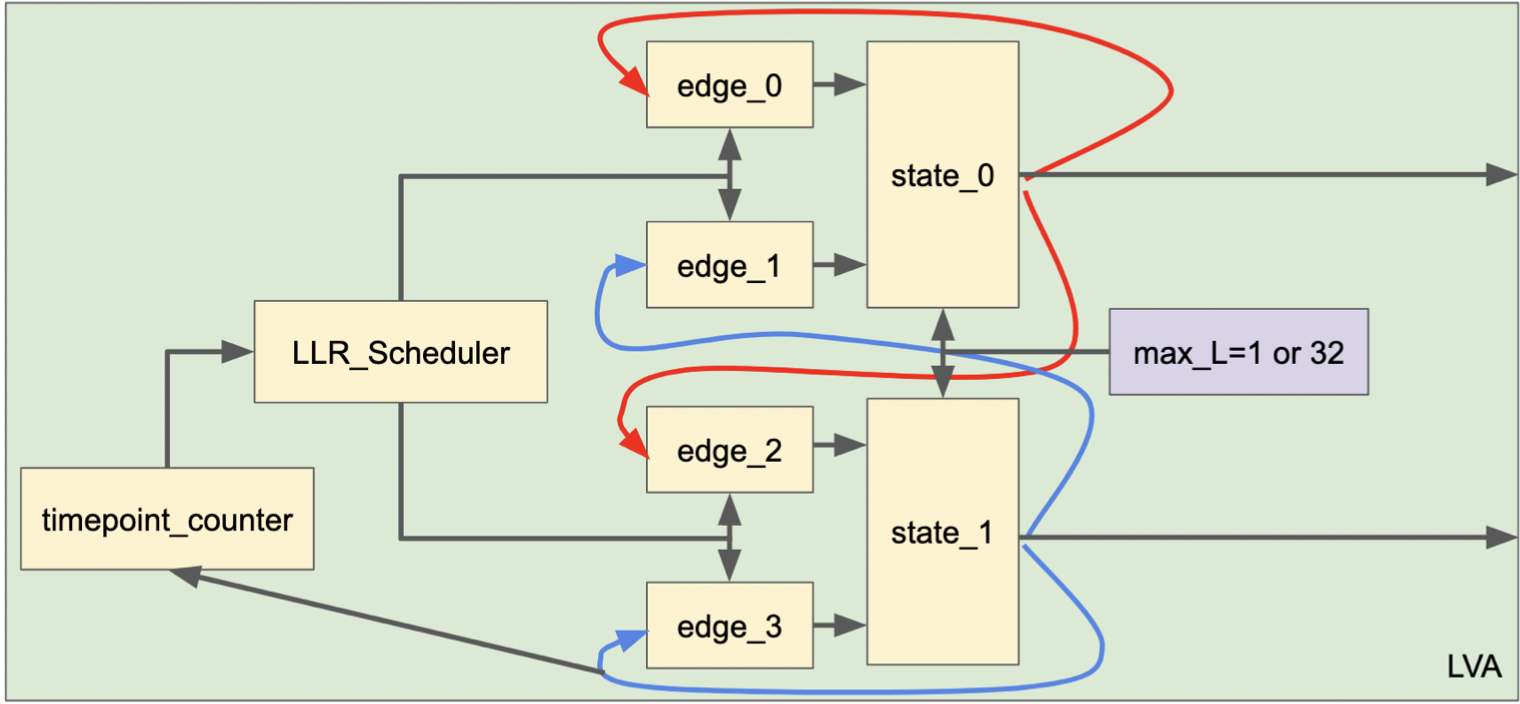
\includegraphics[height=15em]
{Figures/old_lva.png}
\caption[Chester Hulse's design of FPGA LVA]
{Chester Hulse's design of FPGA LVA. Figure taken from \cite{ChesterPaper}}
\label{Figure:DecoderHW:OldLVAModule}
\end{figure}
%%%%%%%%%%%%%%%%%%%%%%%%%%%%%%%%%%%%%%%%%%%%%%%%%%%%%%%%%%%%%%%%%
\TODO{Add cite}

While this design attempts to optimize the parallelism in the decoder, as Hulse mentions, for high state codes it draws too many resources. For example, in the $N=8$ ($S=256 \implies E=512$) case, the FPGA will attempt to synthesize 512 memory blocks which is more than most consumer FPGAs would contain. To synthesize this design on the ZCU106 Evaluation Board (which has 312 BRAM blocks) Distributed RAM was used to fill in the remaining ~200 memory elements (see \Figure~\fref{Figure:DecoderHW:OldUtilization}). Since Distributed RAM uses FPGA LUTs, this introduces routing and timing complications, forcing a lower clock speed, and takes too much space on the board to be reasonable. 

%%%%%%%%%%%%%%%%%%%%%%%%%%%%%%%%%%%%%%%%%%%%%%%%%%%%%%%%%%%%%%%%%
% FIGURE: Decoder HW: Old Design Utilization
\begin{figure}
\centering\CaptionFontSize
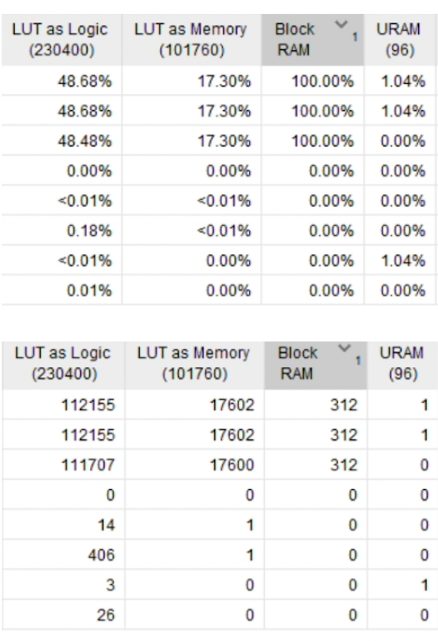
\includegraphics[height=20em]
{Figures/old_design_utilization.png}
\caption[Chester Hulse's design of FPGA LVA hardware utilization]
{Chester Hulse's design of FPGA LVA hardware utilization. Figure taken from \cite{ChesterPaper}}
\label{Figure:DecoderHW:OldUtilization}
\end{figure}
%%%%%%%%%%%%%%%%%%%%%%%%%%%%%%%%%%%%%%%%%%%%%%%%%%%%%%%%%%%%%%%%%
\TODO{cite}

%%%%%%%%%%%%%%%%%%%%%%%%%%%%%%%%%%%%%%%%%%%%%%%%%%%%%%%%%%%%%%%%%
% FIGURE: Decoder HW: FIFO Flushing
\begin{figure}
\centering\CaptionFontSize
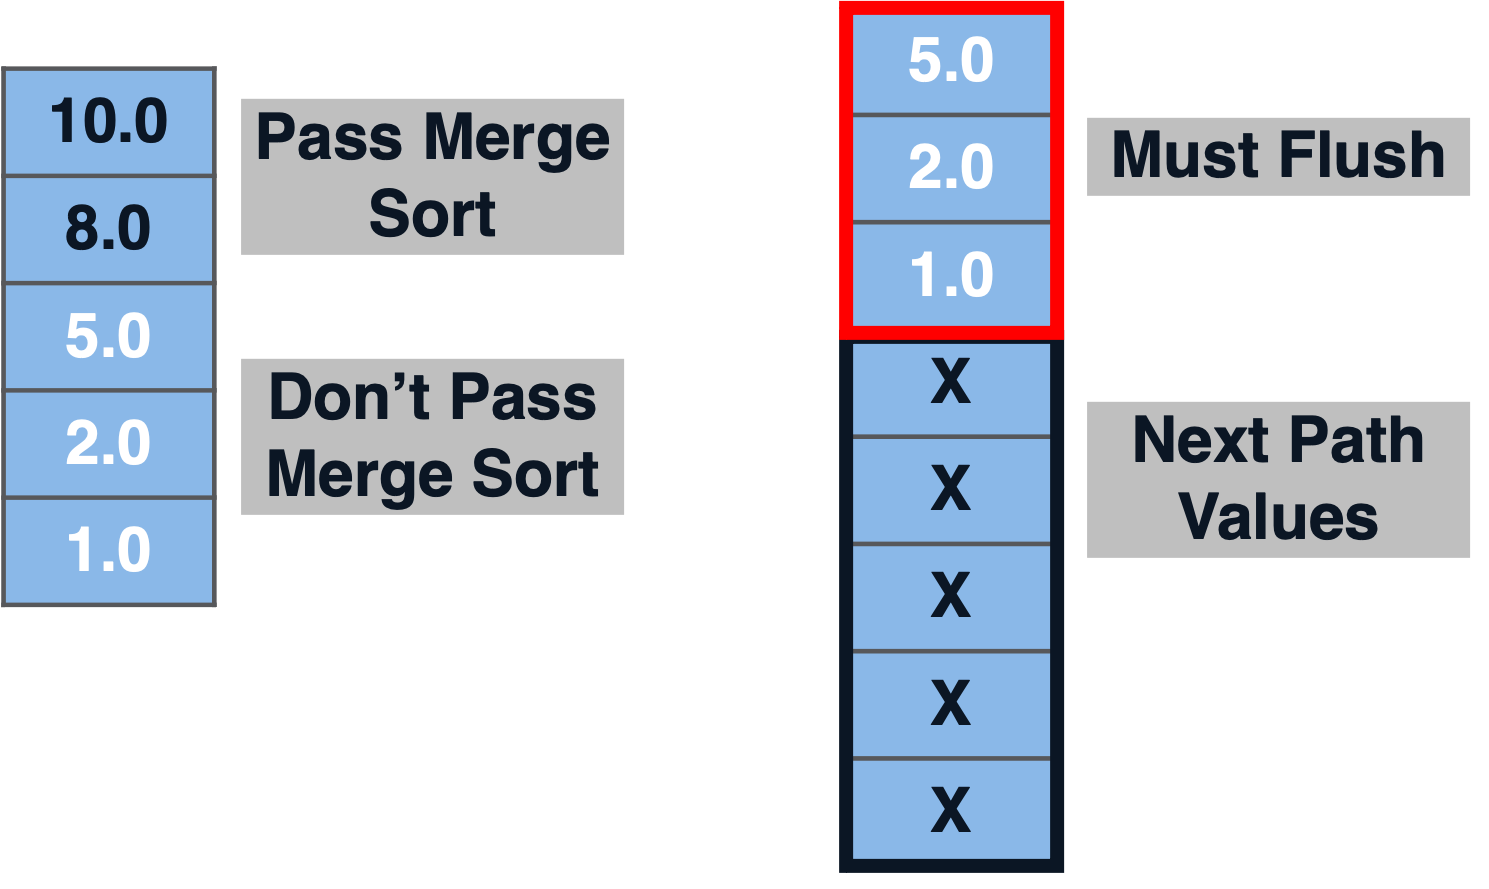
\includegraphics[height=15em]
{Figures/fifo_flush.png}
\caption[Example of FIFO flushing]
{Example of FIFO flushing.}
\label{Figure:DecoderHW:FifoFlushing}
\end{figure}
%%%%%%%%%%%%%%%%%%%%%%%%%%%%%%%%%%%%%%%%%%%%%%%%%%%%%%%%%%%%%%%%%

Additionally, implementing the list storage as a FIFO memory element introduces wasted cycles necessary to “flush” out old unused paths (see \Figure~\fref{Figure:DecoderHW:FifoFlushing}). In a best case scenario, after the $L$ best paths are chosen from the two lists of size $L$, there are still $\frac{L}{2}$ old paths that need to be flushed out of each FIFO before the decoder can move on to the next time point; at worst $L$ paths would need to be flushed.

To address these shortcomings Hulse proposes a change in his original design. Namely, introducing serialism to execution of PLVD per time point instead of attempting to do all state computations in parallel. The amount of parallelism in the implementation can be controlled by the number of BRAMs the user wants the decoder to utilize. In order to still decode high state codes and keep track of the same number of edge paths in the decoding process, each BRAM will have to store more than one edge list. This redesign also allows us to shift to a fixed memory structure instead of FIFO for better performance. The \Figure~\fref{Figure:DecoderHW:NewArchitecture} overviews the redesigned LVA architecture.

%%%%%%%%%%%%%%%%%%%%%%%%%%%%%%%%%%%%%%%%%%%%%%%%%%%%%%%%%%%%%%%%%
% FIGURE: Decoder HW: New Architecture
\begin{figure}
\centering\CaptionFontSize
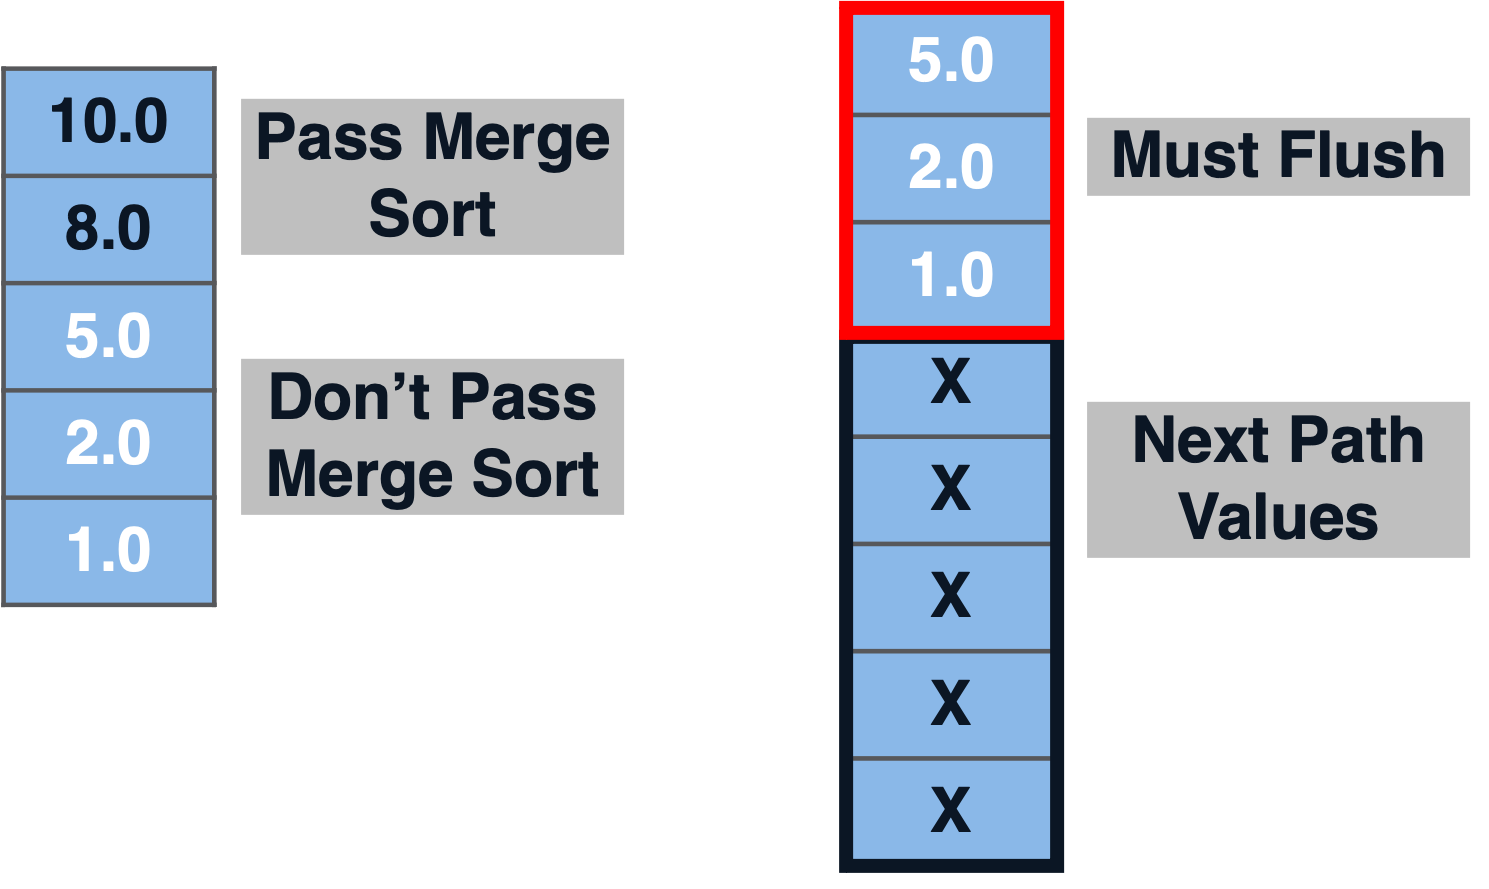
\includegraphics[height=15em]
{Figures/fifo_flush.png}
\caption[Proposed new hardware architecture]
{Proposed new hardware architecture.}
\label{Figure:DecoderHW:NewArchitecture}
\end{figure}
%%%%%%%%%%%%%%%%%%%%%%%%%%%%%%%%%%%%%%%%%%%%%%%%%%%%%%%%%%%%%%%%%
 
Henceforth we will use the parameters in to discuss the new design:
K = number of BRAMs allocated for decoder
S = number of states in the code
E = number of corresponding edges (2*S)

%%%%%%%%%%%%%%%%%%%%%%%%%%%%%%%%%%%%%%%%%%%%%%%%%%%%%%%%%%%%%%%%%
% TABLE: Decoder HW: Parameter Definitions
\begin{table}
\caption[Decoder HW chapter parameters]
{Chapter parameters}
\label{Table:Background:SymbolDefinitions}
\centering\CaptionFontSize
\begin{tabular}{c@{\hspace{1em}}l}
\toprule
Parameter & Definition
\\
\midrule
$K$ & number of BRAMs allocated for decoder
\\
$S$ & number of states in the code
\\
$E$ & number of corresponding edges (2*S)
\\

\bottomrule
\end{tabular}
\end{table}
%%%%%%%%%%%%%%%%%%%%%%%%%%%%%%%%%%%%%%%%%%%%%%%%%%%%%%%%%%%%%%%%%

Since we are no longer doing all state computations in parallel, we must have a system to determine which states we are processing and when. Since we have $K$ BRAMs we are limited to processing $K$ edges at any given moment, implying we can process $\frac{K}{2}$ states in parallel. If we denote a “state iteration” to be completing the computations for these $\frac{K}{2}$ states, then in order to complete all the computations for a given time point we would need $2*S/K = E/K$ state iterations. The new design keeps track of the state iteration using a counter which is utilized by the $\frac{K}{2}$ state and edge modules ( 1 edge module actually keeps track of 2 edges) as described below. Additionally, since we are using fixed memory, there are now bus modules that handle the flow of data in and out of the BRAMs that serve as $K$ multiplexers. 

\subsubsection{Memory and Memory Buses}
One benefit of the FIFO memory mechanism was that doing reads and writes at the same time would require half as much memory space compared to reading and writing from fixed memory. To implement this with fixed memory, the address space of each BRAM needs to be split into two sections. The first section contains the paths that were updated last time point which the decoder reads from. Those paths are used to calculate the metrics for paths in the current time point which are then stored in the second section. Once computations are finished and we move to the next time point, these sections in memory switch roles and the read section becomes the write section and vice versa.

The true bottleneck in the first design was over usage of BRAM blocks without utilizing their depth. This is why despite these changes increasing overall BRAM usage (by a factor of two), the flexibility of the design allows us to more fully utilize memory on board and process high order states.

However, in this design we encounter an interesting problem. Since each edge has a list of size $L$ paths associated with it at every time point, we must distribute the edges (i.e. the list of paths associated with each edge) such that each BRAM has $\frac{E}{K}$ edges associated with it. Furthermore, these edges need to be distributed in such a way that during execution there is always exactly one read and one write per cycle so that we maximize the utilization of the BRAMs available.

To accomplish this, there are two relevant axes of control,

\begin{enumerate}
    \item The choice of states we are processing in parallel
    \item The choice of which edges go into which BRAM
\end{enumerate}



To illustrate this challenge we consider a naive attempt at a solution. If for state $s$ in $[0, S-1]$, $e$ in $[0, E-1]$, and BRAM in $[0, K-1]$.

\begin{enumerate}
    \item We process states $\{0, 1, \ldots, K/2-1\}$, $\{K/2, K/2+1, \ldots, 2K/2-1\}$, $\ldots$ and $\{S-K/2, S-K/2+1 , \ldots, S-1\}$ in parallel.
    \item And we let edge $e$ be in in BRAM $e\%K (mod K)$
\end{enumerate}

Using this method to distribute edges, consider a case where $S = 8$, $E = 16$, and $K = 4$. We will have the following memory layout (\Figure~\fref{Figure:DecoderHW:NaiveMemory}) and execution order (\Figure~\fref{Figure:DecoderHW:NaiveOrdering}).

%%%%%%%%%%%%%%%%%%%%%%%%%%%%%%%%%%%%%%%%%%%%%%%%%%%%%%%%%%%%%%%%%
% FIGURE: Decoder HW: Naive Memory
\begin{figure}
\centering\CaptionFontSize
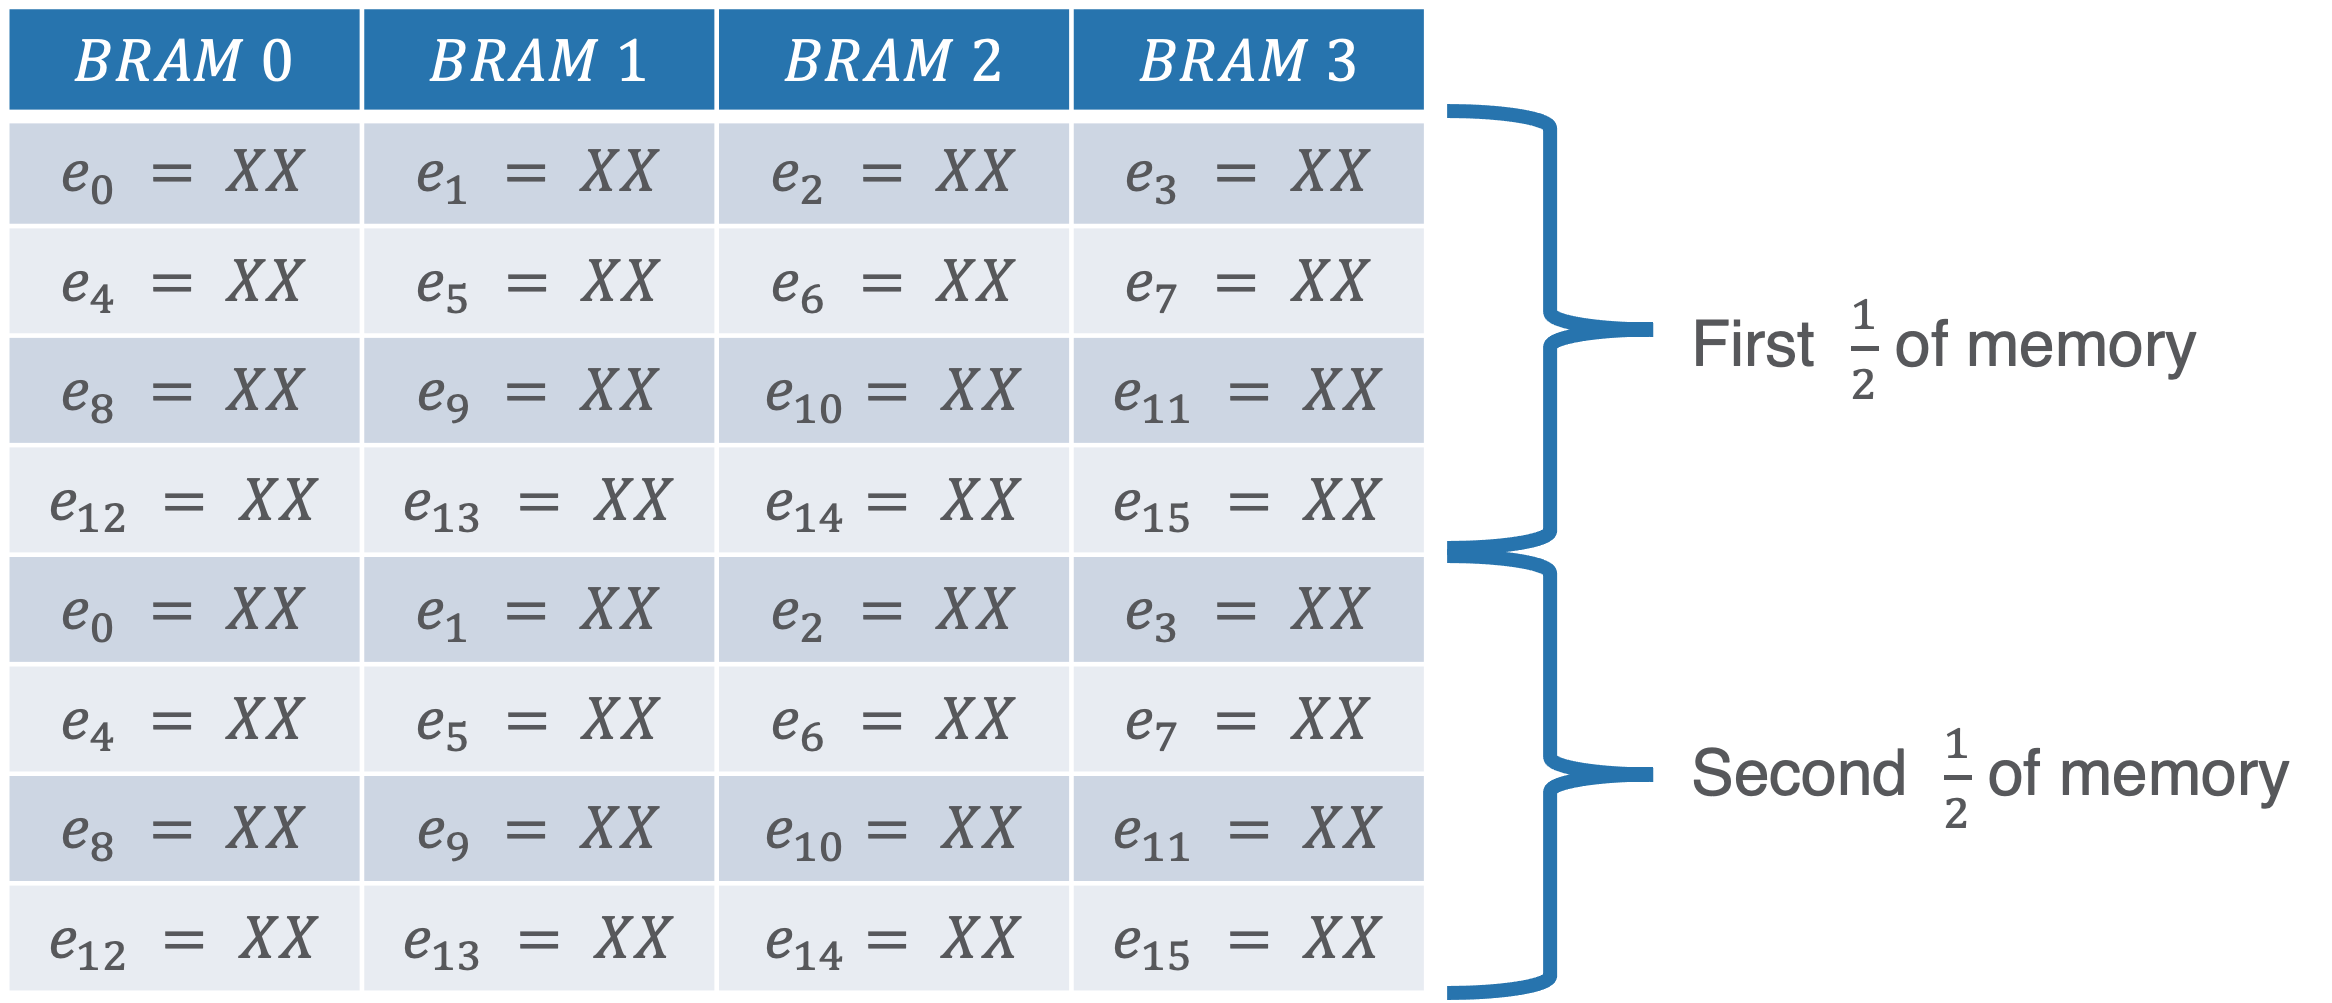
\includegraphics[height=15em]
{Figures/arb_fixed_mem.png}
\caption[Example of an arbitrary fixed memory structure]
{Example of an arbitrary fixed memory structure.}
\label{Figure:DecoderHW:NaiveMemory}
\end{figure}
%%%%%%%%%%%%%%%%%%%%%%%%%%%%%%%%%%%%%%%%%%%%%%%%%%%%%%%%%%%%%%%%%
%%%%%%%%%%%%%%%%%%%%%%%%%%%%%%%%%%%%%%%%%%%%%%%%%%%%%%%%%%%%%%%%%
% FIGURE: Decoder HW: Naive Ordering
\begin{figure}
\centering\CaptionFontSize
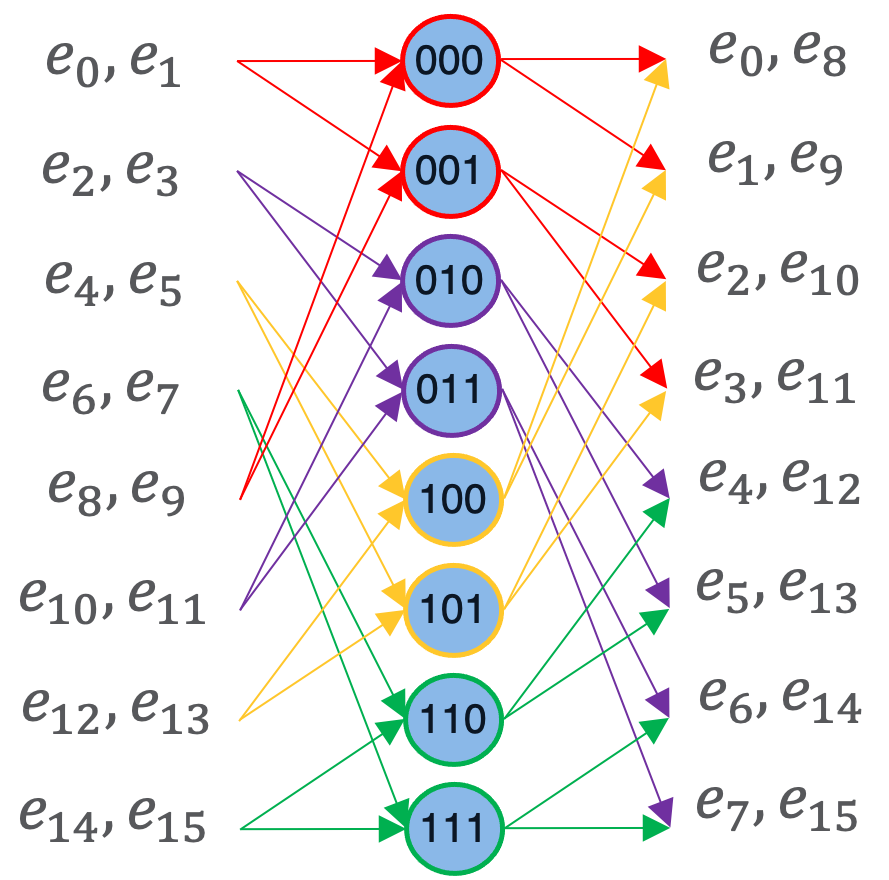
\includegraphics[height=15em]
{Figures/arb_state_ordering.png}
\caption[Example of an arbitrary execution ordering of states]
{Example of an arbitrary execution ordering of states. The execution ordering according to the naive solution would be red $\implies$ purple $\implies$ yellow $\implies$ green}
\label{Figure:DecoderHW:NaiveOrdering}
\end{figure}
%%%%%%%%%%%%%%%%%%%%%%%%%%%%%%%%%%%%%%%%%%%%%%%%%%%%%%%%%%%%%%%%%
In the first “state iteration” of executing the algorithm, we see that since $s_0$ and $s_1$ are being processed, that means that the decoder must read $e_0$, $e_1$, $e_8$, and $e_9$ from memory. However, based on the above memory layout, we must read from BRAM0 and BRAM1 twice and BRAM2 and BRAM3 are left unread. Thus we will inevitably waste cycles by waiting to do two reads, and are letting resources run idle.

Our solution fixes (1) to be the same as in the naive solution, but finds an adequate (2) that allows us to read and write with every BRAM every cycle. 

The solution, interestingly enough, was inspired from the very basics of encoding theory. If we consider each BRAM to have a particular ID represented in binary, then each of the K BRAMs would have a $\log_2(K) = k$ (different $k$ than rate $1/k$) long bit sequence ID. Using this formulation, the problem is redefined as associating each edge with a $k$ bit sequence such that if edges have the same bit sequence they don't share the same read/write state iteration. This association of edges to bits is effectively equivalent to finding a convolutional encoding, and thus we simply need to find a generator polynomial that satisfies the condition. With this realization, testing different strategies to determine a valid (2) became much simpler, and eventually we narrowed down the following encoding to be successful. 
$$G(D) = [ \sum_{n+1-k}^n D^i \quad D^{k-2} \quad \cdots \quad D \quad 1] $$

To prove its validity we simply need to show that for any state iteration, the edges read from memory all come from a unique BRAM and likewise for the edges written to memory. To proceed we will utilize the following 3 lemmas derived from (1) in our solution and general trellis structure observations

\begin{Thm:Lemma}
Due to (1) for arbitrary state iteration $i$, there are $\frac{K}{2}$ states being processed and specifically they are $\{i*K/2, i* K/2+1, \ldots, (i+1)K/2-1\}$. Representing $s$ as a bit sequence $s = (s_1, s_2, \ldots, s_N)$, this implies that every state processed in state iteration $i$ has the same bits $s_1, \ldots, s_{N-k+1}$ (i.e upper $N-k+1$ bits) but unique bit sequence $(s_{N-k+2}, \ldots, s_N)$ (lower $k-1$ bits).
 \label{Thm:Lemma:DecoderHW:Lemma1}
\end{Thm:Lemma}

\begin{Thm:Lemma}
 the edges that are incoming into $s$ are $e_0 = (0, s_1, s_2, \ldots, s_N)$ and $e_1 = (1, s_1, s_2, \ldots, s_N)$.
 \label{Thm:Lemma:DecoderHW:Lemma2}
\end{Thm:Lemma}

\begin{Thm:Lemma}
For any state $s$ in the trellis with bit sequence $(s_1, s_2, \ldots, s_N)$, the outgoing edges are $e_0 = (s_1, s_2, \ldots, s_N, 0)$ and $e_1 = (s_1, s_2, \ldots, s_N, 1)$
\label{Thm:Lemma:DecoderHW:Lemma3}
\end{Thm:Lemma}

\begin{Thm:Proposition}
The combination of (1) and (2) successfully label read edges and write edges such that every state iteration, there is exactly one read and one write from every BRAM.
\label{Thm:Proposition:DecoderHW:Prop1}
\end{Thm:Proposition}

\textbf{Proof of Proposition}

\underline{State Iteration Reads}: To prove our encoding successfully labels edges read at the same time differently, we split the set edges read from memory in an arbitrary state iteration into two cases: If two edges in set enter the same state and if they enter different states. 

In the case where two edges being read from memory are incoming to two on different states by \Lemma~\mref{Thm:Lemma:DecoderHW:Lemma2} $e^i = (e^i_1, s^i_1, s^i_2, \ldots, s^i_N)$ and $e^j = (e^j_1, s^j_1, s^j_2, \ldots, s^j_N)$. (2) necessarily gives the edges different encodings (BRAM IDs) since \Lemma~\mref{Thm:Lemma:DecoderHW:Lemma1} tells us the lower $k-1$ bits of s are distinct. In the other case, \Lemma~\mref{Thm:Lemma:DecoderHW:Lemma2} suggests that if two edges being read enter the same state $s$ then they must be of the form $e^i=(0, s_1, \ldots, s_N)$ and e$^j=(1, s_1, \ldots, s_N)$. Thus, the bottom $k-1$ bits of their encodings will be equivalent (properly), however, the evaluation of (2) to obtain the encoding MSB will be different since $(e^i_1) \neq e^j_1$ while $(e^i_2, \ldots, e^i_N-k+2) = (e^j_2, \ldots, e^j_N-k+2)$. In every case, the encoding procedure (2) produces different BRAM IDs. 

\underline{State Iteration Writes}: We take a similar approach to proving the encoding successfully labels write edges and split cases into edges exiting the different nodes and exiting the same node. 

\Lemma~\mref{Thm:Lemma:DecoderHW:Lemma3} implies two edges exiting the same node are of the form $e^i = (s_1, \ldots, s_N, 0)$ and $e^j = (s_1, \ldots, s_N, 1)$. Applying (2) to these edges, we immediately get different encodings since the LSB of the edges are different. For two edges exiting different states, \Lemma~\mref{Thm:Lemma:DecoderHW:Lemma3} implies $e^i = (s^i_1, \ldots, s^i_N, e^i_N)$ and $e^j = (s^j_1, \ldots, s^j_N, e^j_N)$. If $s^i_{N-k+2} = s^j_{N-k+2}$ then \Lemma~\mref{Thm:Lemma:DecoderHW:Lemma1} implies that the middle $k-2$ bits of $e^i$ and $e^j$’s encoding are different. If $s^i_{N-k+2} \neq s^j_N{-k+2}$ then the MSB of $e^i$ and $e^j$’s encoding are different since \Lemma~\mref{Thm:Lemma:DecoderHW:Lemma1} states that upper ${N-k+1}$ bits in the expressions (sum) and (sum) are the same. In every case, the encoding procedure (2) produces different BRAM IDs.

We have proven the solution (1) \& (2) solves the issue of BRAM to edge allocation, however, how about the location of edges within a particular BRAM? An interesting corollary to \Lemma~\mref{Thm:Lemma:DecoderHW:Lemma1} is that if two states $s^i$ and $s^j$ are processed in different state iterations, then their first $N-k+1$ bit sequences will be unique, i.e. $(s^i_1, \ldots, s^i_N-k+1) \neq (s^i_1, \ldots, s^i_{N-k+1})$. Thus we choose to start the list of arbitrary edges $e = (e_1, \ldots, e_N+1)$ at address $(e_1, \ldots, e_N-k+1, 0, \ldots, 0)$ where the number of inserted 0s is dependent on the maximum list size desired. This way, any edge processed in a different state iteration that shares a BRAM with e will necessarily have a different address for its list. Furthermore, edges within e’s state iteration might have the same address, but will be in different BRAMs. \Figure~\fref{Figure:DecoderHW:NewMemory} is an example of using this storage method for the K=4, S=8 case.

%%%%%%%%%%%%%%%%%%%%%%%%%%%%%%%%%%%%%%%%%%%%%%%%%%%%%%%%%%%%%%%%%
% FIGURE: Decoder HW: New Memory
\begin{figure}
\centering\CaptionFontSize
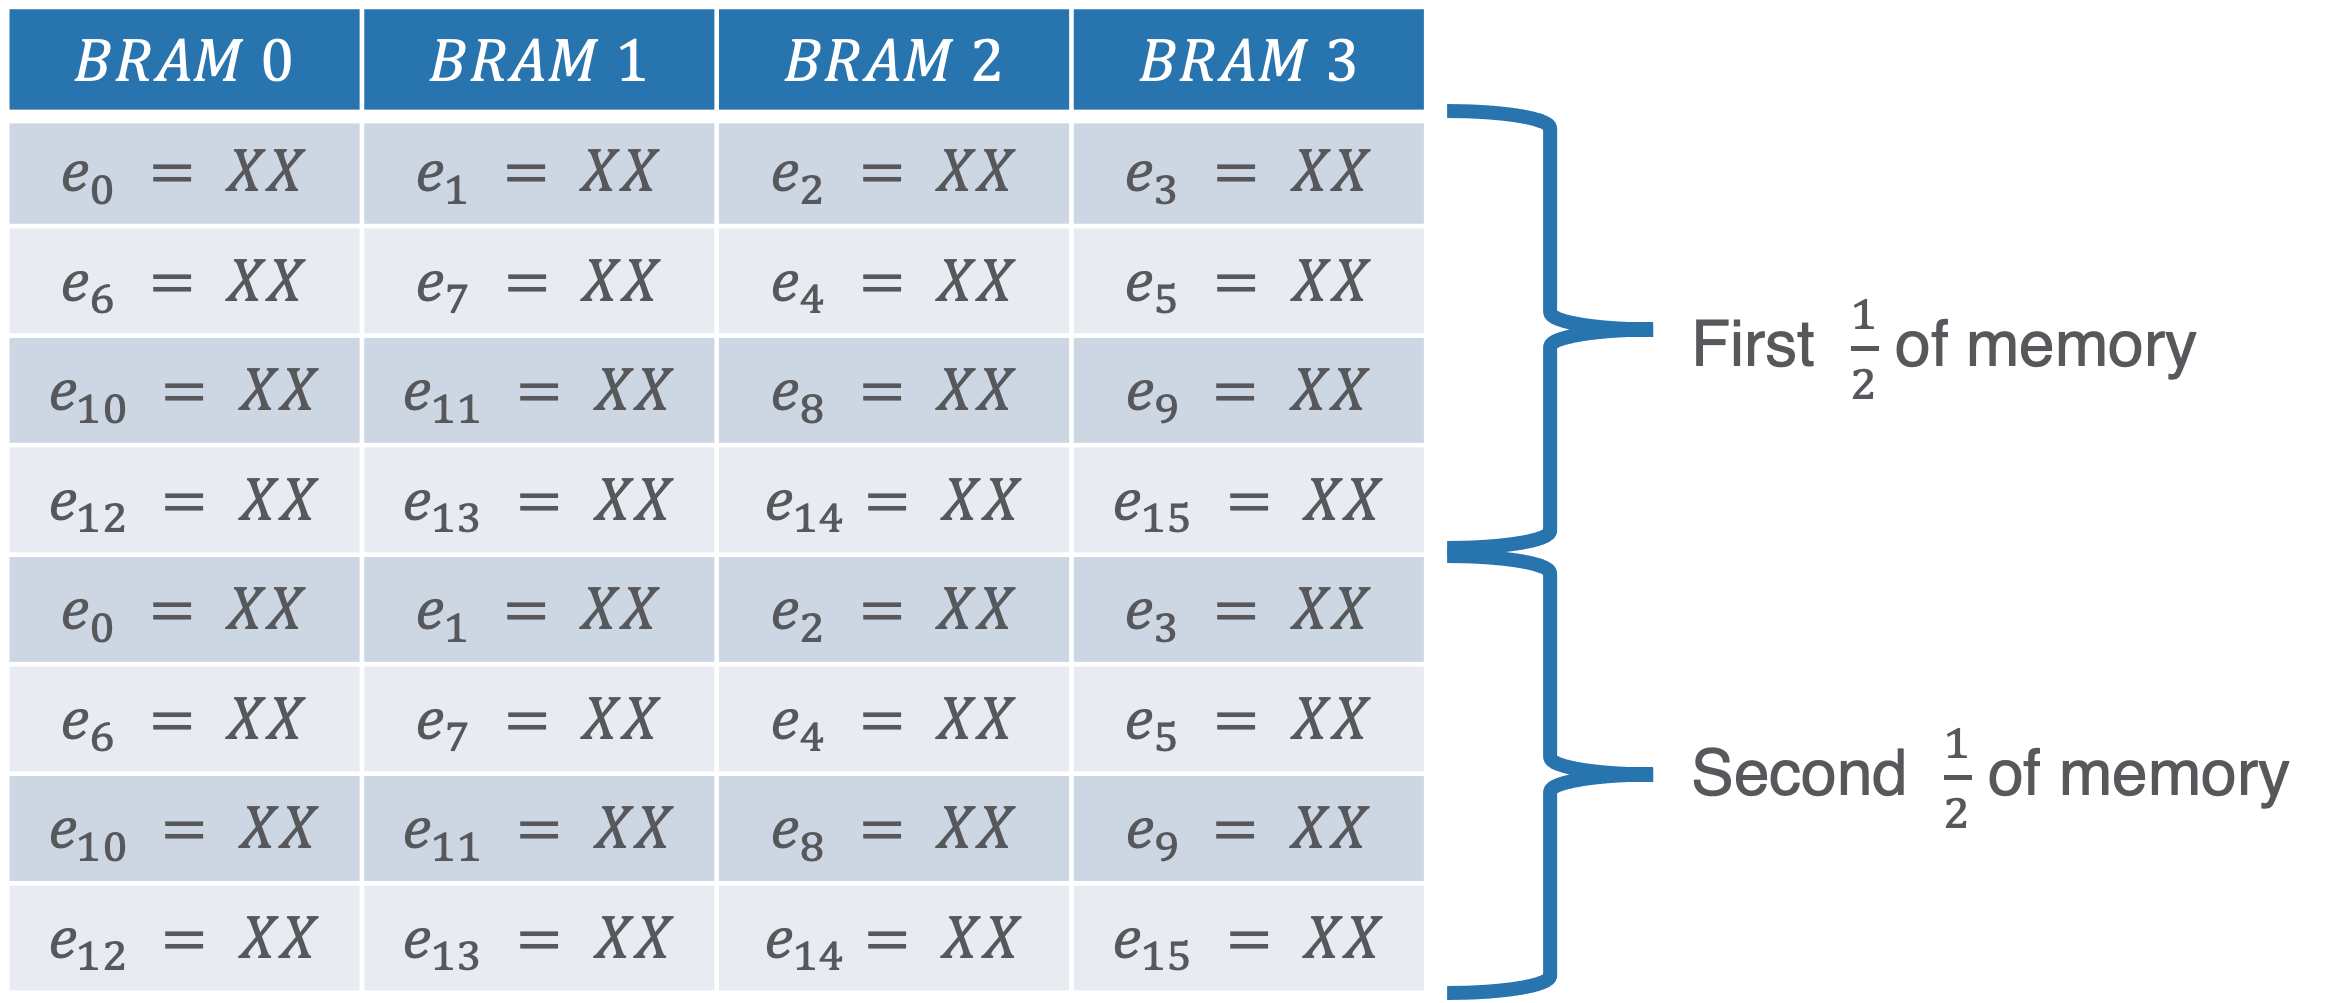
\includegraphics[height=15em]
{Figures/new_fixed_mem.png}
\caption[Example of new fixed memory structure]
{Example of new fixed memory structure.}
\label{Figure:DecoderHW:NewMemory}
\end{figure}
%%%%%%%%%%%%%%%%%%%%%%%%%%%%%%%%%%%%%%%%%%%%%%%%%%%%%%%%%%%%%%%%% 

Since we are using multiple addressable BRAMs to implement this design, a bus is necessary to serve as a multiplexor of BRAMs and handle the flow of data from memory to computation modules. Together, the memory and bus modules enable the decoder to efficiently read and write $K$ data streams as long as it’s provided with the proper BRAM IDs and addresses associated with the data being streamed.

We’ve established memory allocation for the list of paths in the decoder, this alteration somewhat forces changes in the state and edge modules from Hulse’s design.

\subsubsection{State Module}

Instead of instantiating $S$ state modules, LVA now instantiates $\frac{K}{2}$ modules each with a unique parameter STATE\_NUMBER that ranges from 0 to K/2-1. This parameter represents which “relative” state the module is processing each state iteration. As an input to the module are two AXI-LITE streams that correspond to the state’s two incoming edges. The iteration counter is also fed as an input (ITERATION) to the module and is used in conjunction with STATE\_NUMBER to calculate the base addresses of the two incoming lists. 
Using notation from the last section, \Lemma~\mref{Thm:Lemma:DecoderHW:Lemma1} implies that the states processed at ITERATION are s = (ITERATION, STATE\_NUMBER) where STATE\_NUMBER and ITERATION are respectively $k-1$ and $N-k+1$ bit sequences.

Thus, for the state module with parameter STATE\_NUMBER in ITERATION, \Lemma~\mref{Thm:Lemma:DecoderHW:Lemma2} and our methods for computing an edge’s BRAM ID and address give us simple hardware implementations that determine the base addresses of the lists required.

\begin{itemize}
    \item Top incoming edge:
    \begin{itemize}
        \item BRAM: G({0, ITERATION, STATE_NUMBER})
        \item address: (0, ITERATION>>1)<<$\log_2(Lmax)$
    \end{itemize}
    \item Bottom incoming edge:
        \begin{itemize}
        \item BRAM: G({1, ITERATION, STATE_NUMBER})
        \item address: (1, ITERATION>>1)<<$\log_2(Lmax)$
    \end{itemize}
\end{itemize}

Note that $G(D)$ is very efficient to do in hardware, only requiring $N-k+1$ XORs.

To execute the function of filtering the two incoming lists, each cycle the state module simply needs to read the data at the two computed base addresses, compare the two metrics, output the path with the better metric, and then increment the address that had that path by 1. This is repeated until either all valid paths have been read or $Lmax$ paths were outputted.

\subsubsection{Edge Module}
The changes to the edge modules are similar to the state module. Each of the $\frac{L}{2}$ edge modules use their unique STATE\_NUMBER and input ITERATION to calculate the base address of which two edges it is writing to. Its input is a stream of paths from its corresponding state module, and it outputs two AXI-LITE streams with updated path objects with metrics representing the state’s output edges. Furthermore, it inputs the LLRs associated with the received codeword for that time point.

The computations for an edge modules write locations are

\begin{itemize}
    \item Top incoming edge:
    \begin{itemize}
        \item BRAM: G({ITERATION, STATE_NUMBER, 0})
        \item address: (ITERATION)<<$\log_2(Lmax)$
    \end{itemize}
    \item Bottom incoming edge:
        \begin{itemize}
        \item BRAM: G({ITERATION, STATE_NUMBER, 1})
        \item address: (ITERATION)<<$\log_2(Lmax)$
    \end{itemize}
\end{itemize}

The edge module performs the metric calculations as detailed earlier by using STATE\_NUMBER and ITERATION to find the correct “mask” for one of the outgoing edges and using it to calculate the metric update $X$. The output path object for one of the edges will be the input path object with $X$ added to the metric, and the other output will subtract $X$ from the input path metric. These outputs will be AXI-LITE streams that write to the base addresses above in memory where every cycle the address increments by one.

\subsection{Projected Performance and Future Work}
Currently we are still in the process of implementing these changes to the design and running simulation/verification tests on the updated modules. Once complete, we aim to ensure these designs are synthesizable on board and compare resource utilization to the previous design and what is expected.

Since BRAMs used for memory is a user configurable parameter in our design ($K$), we expect BRAMs used to be $~K$. Thus, Distributed RAM instantiation should be 0 since they won't have to be used as BRAM substitutes anymore. Overall we also expect less arithmetic/logic since they correlate to the number of instantiated state and edge modules which scale with $K$. 

In terms of compute time, we expect the trellis propagation portion changing from finishing in $O(L*T)$ cycles to finishing in $O(2*S*L*T/K)$ cycles.

Once implemented and tested, this accelerated PLVD can be used as a computational core for simulating and implementing modifications to PLVD such as the work done by Jacob King \cite{king2023design}. Furthermore, accelerating PLVD allows us to compare its performance as a decoding scheme against other decoders such as SVLD and any future decoding algorithms.

\TODO{cite properly}

